% ============================================================
% Plantilla de Ejemplo: Figura / Ilustración (Normas APA 7)
% Proyecto de Grado BTH — Modalidad Innovación Tecnológica
% ============================================================
%
% Este archivo muestra la estructura formal de una figura según
% el estándar APA 7ma Edición:
%   1. Rótulo y Título ARRIBA de la ilustración (\caption).
%   2. Contenido visual centrado (\centering y \includegraphics).
%   3. Nota al pie ABAJO con la fuente o aclaración (\notafigura).
%
% Para incluir esta figura en cualquier capítulo o sección, use:
%   % ============================================================
% Plantilla de Ejemplo: Figura / Ilustración (Normas APA 7)
% Proyecto de Grado BTH — Modalidad Innovación Tecnológica
% ============================================================
%
% Este archivo muestra la estructura formal de una figura según
% el estándar APA 7ma Edición:
%   1. Rótulo y Título ARRIBA de la ilustración (\caption).
%   2. Contenido visual centrado (\centering y \includegraphics).
%   3. Nota al pie ABAJO con la fuente o aclaración (\notafigura).
%
% Para incluir esta figura en cualquier capítulo o sección, use:
%   % ============================================================
% Plantilla de Ejemplo: Figura / Ilustración (Normas APA 7)
% Proyecto de Grado BTH — Modalidad Innovación Tecnológica
% ============================================================
%
% Este archivo muestra la estructura formal de una figura según
% el estándar APA 7ma Edición:
%   1. Rótulo y Título ARRIBA de la ilustración (\caption).
%   2. Contenido visual centrado (\centering y \includegraphics).
%   3. Nota al pie ABAJO con la fuente o aclaración (\notafigura).
%
% Para incluir esta figura en cualquier capítulo o sección, use:
%   % ============================================================
% Plantilla de Ejemplo: Figura / Ilustración (Normas APA 7)
% Proyecto de Grado BTH — Modalidad Innovación Tecnológica
% ============================================================
%
% Este archivo muestra la estructura formal de una figura según
% el estándar APA 7ma Edición:
%   1. Rótulo y Título ARRIBA de la ilustración (\caption).
%   2. Contenido visual centrado (\centering y \includegraphics).
%   3. Nota al pie ABAJO con la fuente o aclaración (\notafigura).
%
% Para incluir esta figura en cualquier capítulo o sección, use:
%   \input{imagenes/figura_ejemplo}
% O utilice el comando semántico directo:
%   \incluirfigura{diagrama_proceso_ejemplo.png}{Título}{fig:clave}{Nota}

\begin{figure}[htbp]
    \centering
    \caption{Diagrama de flujo del proceso de transformación e innovación técnica.}
    \label{fig:diagrama_proceso_innovacion}
    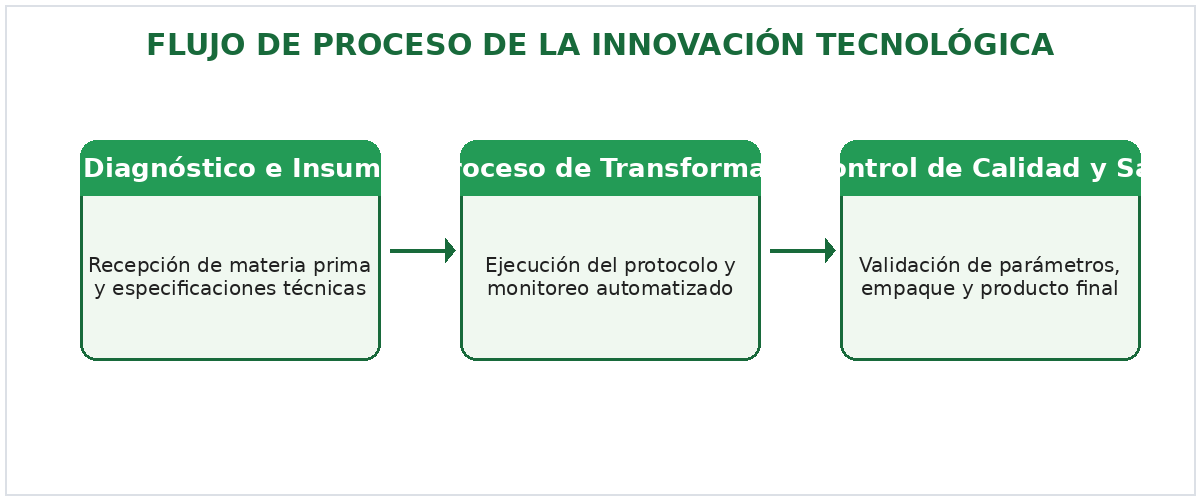
\includegraphics[width=\anchuraimagenpredeterminada]{diagrama_proceso_ejemplo.png}
    \notafigura{Elaboración propia con base en el protocolo de desarrollo operativo.}
\end{figure}

% O utilice el comando semántico directo:
%   \incluirfigura{diagrama_proceso_ejemplo.png}{Título}{fig:clave}{Nota}

\begin{figure}[htbp]
    \centering
    \caption{Diagrama de flujo del proceso de transformación e innovación técnica.}
    \label{fig:diagrama_proceso_innovacion}
    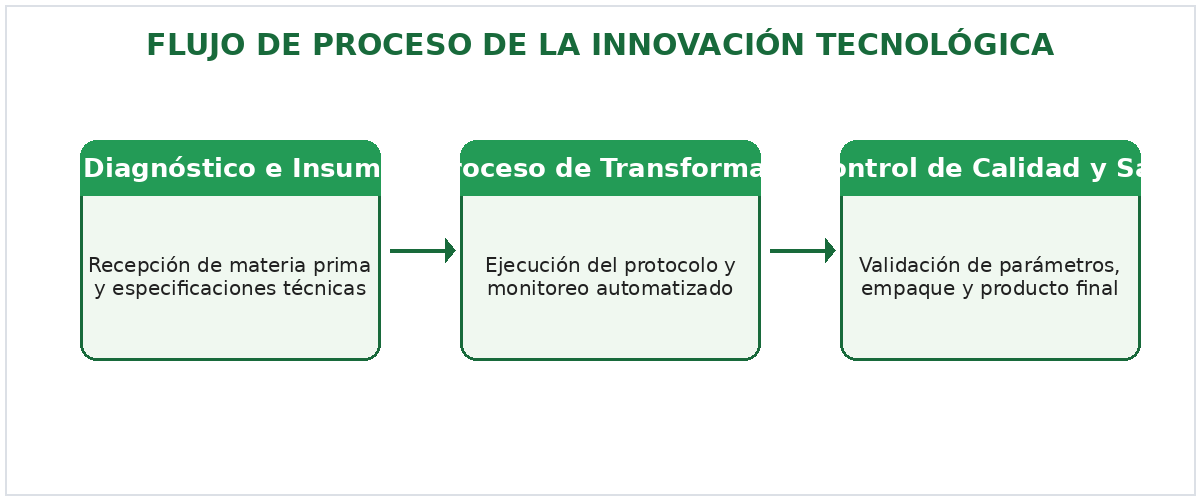
\includegraphics[width=\anchuraimagenpredeterminada]{diagrama_proceso_ejemplo.png}
    \notafigura{Elaboración propia con base en el protocolo de desarrollo operativo.}
\end{figure}

% O utilice el comando semántico directo:
%   \incluirfigura{diagrama_proceso_ejemplo.png}{Título}{fig:clave}{Nota}

\begin{figure}[htbp]
    \centering
    \caption{Diagrama de flujo del proceso de transformación e innovación técnica.}
    \label{fig:diagrama_proceso_innovacion}
    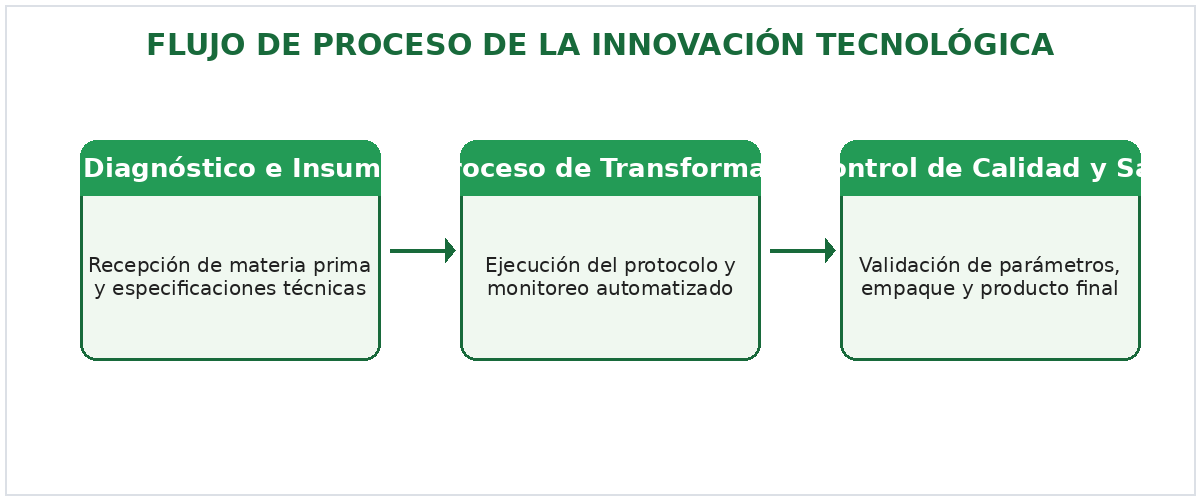
\includegraphics[width=\anchuraimagenpredeterminada]{diagrama_proceso_ejemplo.png}
    \notafigura{Elaboración propia con base en el protocolo de desarrollo operativo.}
\end{figure}

% O utilice el comando semántico directo:
%   \incluirfigura{diagrama_proceso_ejemplo.png}{Título}{fig:clave}{Nota}

\begin{figure}[htbp]
    \centering
    \caption{Diagrama de flujo del proceso de transformación e innovación técnica.}
    \label{fig:diagrama_proceso_innovacion}
    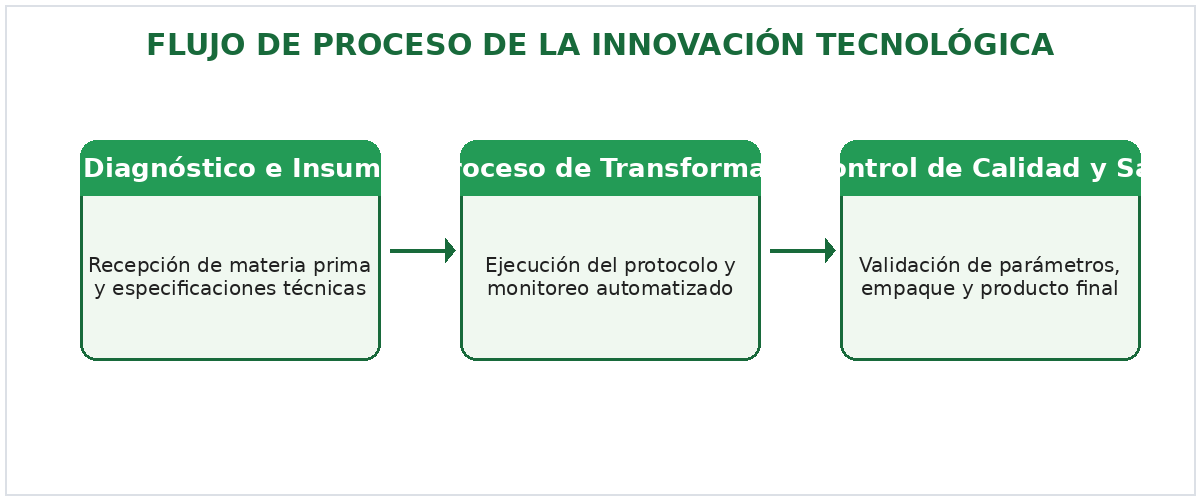
\includegraphics[width=\anchuraimagenpredeterminada]{diagrama_proceso_ejemplo.png}
    \notafigura{Elaboración propia con base en el protocolo de desarrollo operativo.}
\end{figure}
